Cette section explique comment j'ai organisé mon travail et quels sont les outils que j'ai utilisés.

\section{Github}
Bien qu'un \emph{repository} Github existe déjà, j'ai fait le choix de partir d'une base vierge. J'ai donc créé un nouveau \emph{repository open source} ainsi que deux nouveaux projets pour le \emph{frontend} et le \emph{backend}. Il s'agit donc d'un \emph{mono-repo}, c'est quand un seul \emph{repository} contient plusieurs projets distinct. En effet, il me semblait plus simple de partir d'une base nouvelle et de réutiliser les éléments du projet existant au fur et à mesure. De plus, cela me permet d'avoir une meilleure maîtrise du projet dans son entièreté.

Une fois le travail terminé, il sera intéressant faire une \emph{Pull Request} sur le \emph{repository} de base afin de toujours avoir accès à toutes les versions et commit ce projet dans sa totalité.

Ce \emph{repository} est accessible \href{https://github.com/Marinlestylo/h-quiz}{en cliquant ici}. Il est structuré de la manière suivante :
\begin{itemize}
    \item \textbf{Un dossier "api-backend"} : contient le code du de notre API.
    \item \textbf{Un dossier "frontend"} : contient le code de l'interface utilisateur.
    \item \textbf{Un fichier .gitignore} : Explicite tous les fichiers qui ne doivent pas être poussés sur GitHub.
    \item \textbf{Un fichier README.md} : Explique les technologies et comment lancer le projet.
\end{itemize}

\subsection{README}
Comme mentionné dans le premier chapitre, le manque de documentation rend ce projet plus difficile à reprendre. C'est pourquoi j'ai décidé d'avoir un \emph{README} complet et précis permettant une reprise facilité du projet. On y trouve également des informations concernant le \emph{workflow} de ce projet ainsi que son déploiement.

\subsection{User stories}
GitHub offre un système d'issue qui permet de signaler qu'une fonctionnalité doit être réalisée. Cela permet de garder une trace de ce qui doit être fait et de les marquer comme finie, une fois implémentée. Cela permet également de voir l'avancement du projet. Vous pouvez trouver la liste de toutes les issues ouvertes \href{https://github.com/Marinlestylo/h-quiz/issues}{ici}. Il est important de noter qu'à ce stade du projet, les issues ne sont pas encore toutes écrites.

GitHub nous offre également une vue d'ensemble de toutes ces issues. En effet, grâce à la fonctionnalité \emph{Projects}, nous pouvons créer des projets et y ajouter des issues. Avec la vue "tableau", nous avons une vue d'ensemble de toutes les issues et trois colonnes : \emph{To do}, \emph{In progress} et \emph{Done}. On peut donc savoir ce qui est en cours de réalisation. Ces fonctionnalités sont incroyablement utiles lorsqu'on travaille en équipe. Même si elles sont moins importantes quand on est seul sur un projet, cela nous permet de mesurer l'avancement du projet.

Je n'ai finalement pas vraiment utilisé ces \emph{issues} sur github. Je suis plutôt parti sur une copie du cahier des charges avec tous les objectifs à atteindre et je les coloriais en une couleur lorsqu'ils étaient atteints. Cela m'a permis de visualiser l'ensemble des objectifs et d'être sûr d'en oublier aucun.

\subsection{Branches et commits}
Pour ce qui est de la gestion des branches, j'ai décidé de rester très simple et de n'utiliser que deux branches : \emph{main} et \emph{dev}. La branche \emph{main} est la branche principale. Elle doit être fonctionnelle à tout moment. C'est également la branche qui sera utilisée pour le déploiement du projet.

La branche \emph{dev}, quant à elle, sera celle où je vais développer les fonctionnalités. Lorsque plusieurs fonctionnalités sont implémentées et sont entièrement fonctionnelles, je fusionne les branches dans \emph{main}.

Je n'ai pas utilisé cette méthodologie de travail dès le début du projet. En effet, j'ai commencé par travailler directement sur la branche \emph{main} afin d'avoir une base solide pour le projet. Une fois que l'API, sa connexion avec Keycloak et les communications entre le \emph{frontend} et le \emph{backend} étaient fonctionnelles, j'ai créé la branche \emph{dev} et j'ai adopté cette méthodologie de travail.

Pour ce qui est des \emph{commits}, je me base sur les \emph{Conventional Commits} \cite{ConventionalCommits}. Plus particulièrement, tous mes \emph{commits} sont écrits en anglais et sont tous préfixés par un type.

Les types que j'utilise sont les suivants :
\begin{itemize}
    \item feat : Une nouvelle fonctionnalité a été ajoutée.
    \item fix : Une erreur a été corrigée.
    \item docs : La documentation a été modifiée.
    \item chore : Création d'un projet ou d'un dossier.
    \item refactor : Refactorisation d'une partie du code.
\end{itemize}

\section{Stratégie de refactoring}

Mon objectif principal était de reconstruire l'application de manière méthodique et progressive, tout en gardant une version fonctionnelle à tout moment. En effet, il était très important pour moi que l'application soit utilisable et puisse facilement être reprise à la fin de mon travail.

Pour cela, j'ai choisi de partir d'une base vierge et d'utiliser les dernières versions de Laravel et Vue.js, afin d'implémenter les fonctionnalités de manière itérative. Cette démarche m'a permis de m'inspirer du travail existant tout en bénéficiant des dernières fonctionnalités de ces technologies.

Une autre décision importante était de refactoriser simultanément le \emph{backend} et le \emph{frontend}. Cette approche me permet de tester directement l'interaction et le bon fonctionnement des deux parties ensemble. Cela évite également d'avoir à revenir sur du code écrit il y a plusieurs semaines, qui serait plus difficile à comprendre. Finalement, cela permet d'avoir une cohérence entre les deux parties et évite d'avoir une API qui contient des fonctionnalités qui ne sont pas utilisées par le \emph{frontend}.

\section{Planification}
Voici la planification qui a été faite au début de ce travail :

\begin{center}
    \begin{figure}[H]
        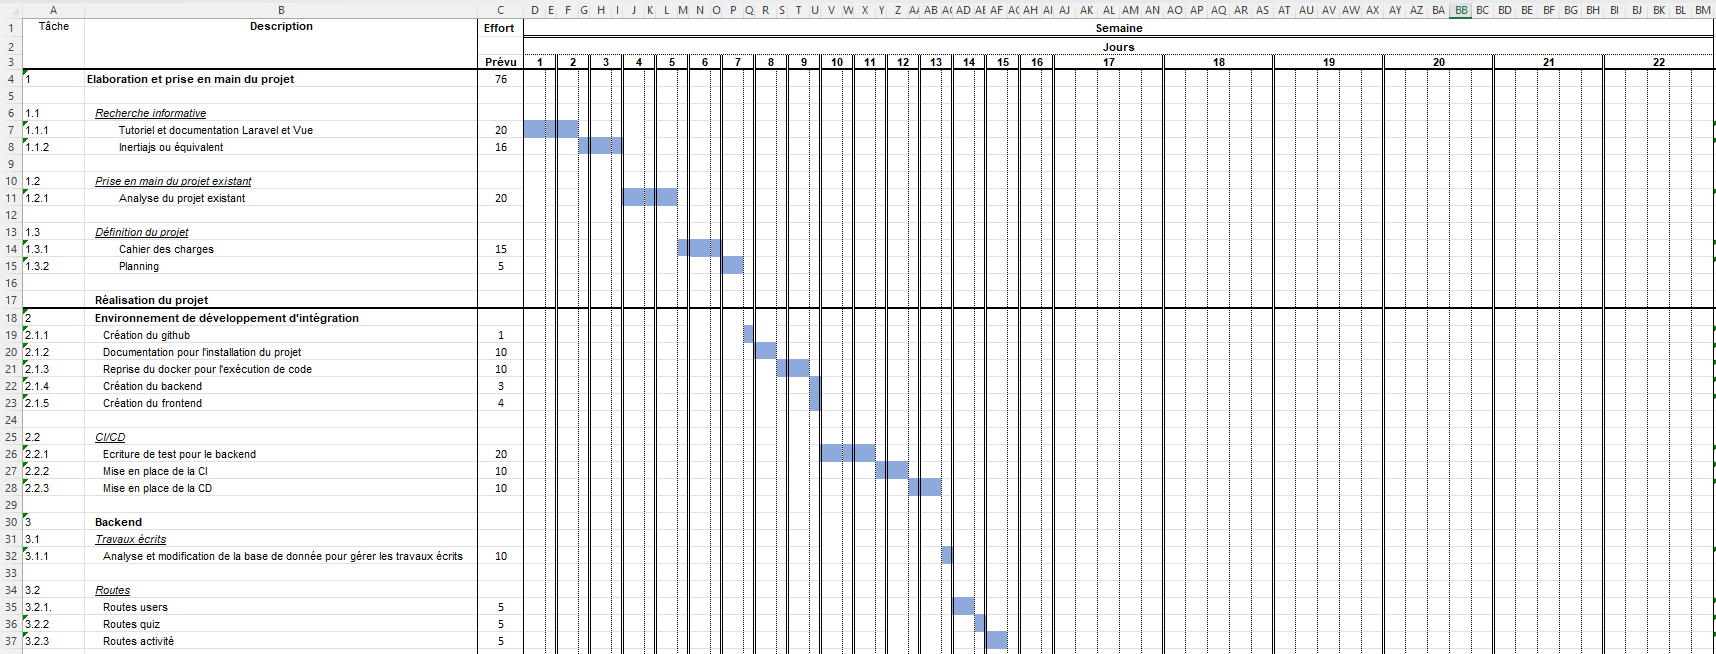
\includegraphics[width=14cm]{./assets/figures/planif1.png}
        \caption{Planification partie 1}
    \end{figure}
\end{center}

\begin{center}
    \begin{figure}[H]
        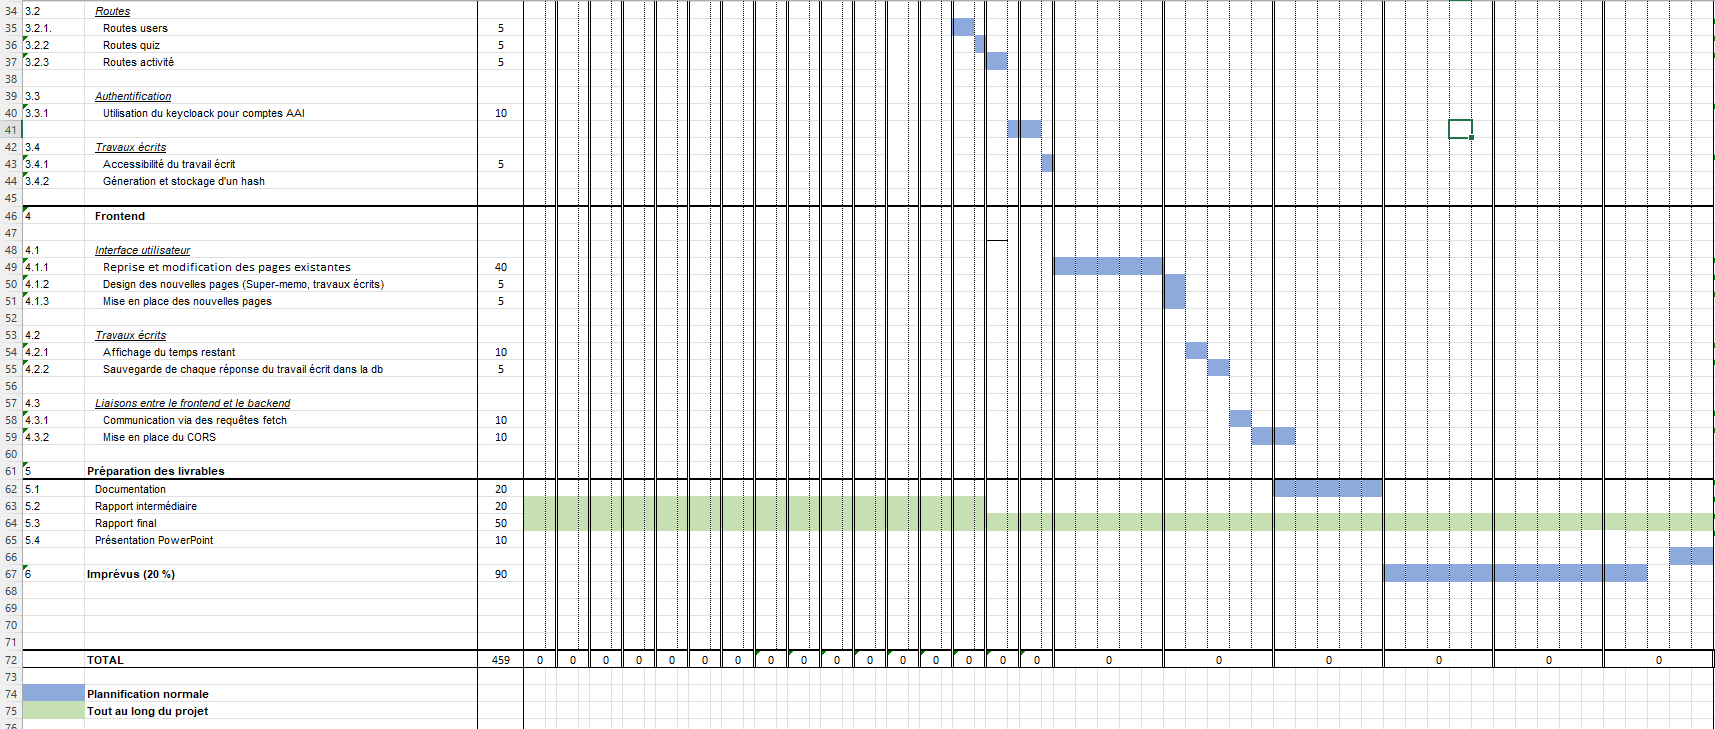
\includegraphics[width=14cm]{./assets/figures/planif2.png}
        \caption{Planification partie 2}
    \end{figure}
\end{center}

Ce document peut également être retrouvé dans les annexes du rapport.